% Options for packages loaded elsewhere
\PassOptionsToPackage{unicode}{hyperref}
\PassOptionsToPackage{hyphens}{url}
\PassOptionsToPackage{dvipsnames,svgnames,x11names}{xcolor}
%
\documentclass[
  letterpaper,
  DIV=11,
  numbers=noendperiod]{scrreprt}

\usepackage{amsmath,amssymb}
\usepackage{lmodern}
\usepackage{iftex}
\ifPDFTeX
  \usepackage[T1]{fontenc}
  \usepackage[utf8]{inputenc}
  \usepackage{textcomp} % provide euro and other symbols
\else % if luatex or xetex
  \usepackage{unicode-math}
  \defaultfontfeatures{Scale=MatchLowercase}
  \defaultfontfeatures[\rmfamily]{Ligatures=TeX,Scale=1}
\fi
% Use upquote if available, for straight quotes in verbatim environments
\IfFileExists{upquote.sty}{\usepackage{upquote}}{}
\IfFileExists{microtype.sty}{% use microtype if available
  \usepackage[]{microtype}
  \UseMicrotypeSet[protrusion]{basicmath} % disable protrusion for tt fonts
}{}
\makeatletter
\@ifundefined{KOMAClassName}{% if non-KOMA class
  \IfFileExists{parskip.sty}{%
    \usepackage{parskip}
  }{% else
    \setlength{\parindent}{0pt}
    \setlength{\parskip}{6pt plus 2pt minus 1pt}}
}{% if KOMA class
  \KOMAoptions{parskip=half}}
\makeatother
\usepackage{xcolor}
\setlength{\emergencystretch}{3em} % prevent overfull lines
\setcounter{secnumdepth}{5}
% Make \paragraph and \subparagraph free-standing
\ifx\paragraph\undefined\else
  \let\oldparagraph\paragraph
  \renewcommand{\paragraph}[1]{\oldparagraph{#1}\mbox{}}
\fi
\ifx\subparagraph\undefined\else
  \let\oldsubparagraph\subparagraph
  \renewcommand{\subparagraph}[1]{\oldsubparagraph{#1}\mbox{}}
\fi


\providecommand{\tightlist}{%
  \setlength{\itemsep}{0pt}\setlength{\parskip}{0pt}}\usepackage{longtable,booktabs,array}
\usepackage{calc} % for calculating minipage widths
% Correct order of tables after \paragraph or \subparagraph
\usepackage{etoolbox}
\makeatletter
\patchcmd\longtable{\par}{\if@noskipsec\mbox{}\fi\par}{}{}
\makeatother
% Allow footnotes in longtable head/foot
\IfFileExists{footnotehyper.sty}{\usepackage{footnotehyper}}{\usepackage{footnote}}
\makesavenoteenv{longtable}
\usepackage{graphicx}
\makeatletter
\def\maxwidth{\ifdim\Gin@nat@width>\linewidth\linewidth\else\Gin@nat@width\fi}
\def\maxheight{\ifdim\Gin@nat@height>\textheight\textheight\else\Gin@nat@height\fi}
\makeatother
% Scale images if necessary, so that they will not overflow the page
% margins by default, and it is still possible to overwrite the defaults
% using explicit options in \includegraphics[width, height, ...]{}
\setkeys{Gin}{width=\maxwidth,height=\maxheight,keepaspectratio}
% Set default figure placement to htbp
\makeatletter
\def\fps@figure{htbp}
\makeatother
\newlength{\cslhangindent}
\setlength{\cslhangindent}{1.5em}
\newlength{\csllabelwidth}
\setlength{\csllabelwidth}{3em}
\newlength{\cslentryspacingunit} % times entry-spacing
\setlength{\cslentryspacingunit}{\parskip}
\newenvironment{CSLReferences}[2] % #1 hanging-ident, #2 entry spacing
 {% don't indent paragraphs
  \setlength{\parindent}{0pt}
  % turn on hanging indent if param 1 is 1
  \ifodd #1
  \let\oldpar\par
  \def\par{\hangindent=\cslhangindent\oldpar}
  \fi
  % set entry spacing
  \setlength{\parskip}{#2\cslentryspacingunit}
 }%
 {}
\usepackage{calc}
\newcommand{\CSLBlock}[1]{#1\hfill\break}
\newcommand{\CSLLeftMargin}[1]{\parbox[t]{\csllabelwidth}{#1}}
\newcommand{\CSLRightInline}[1]{\parbox[t]{\linewidth - \csllabelwidth}{#1}\break}
\newcommand{\CSLIndent}[1]{\hspace{\cslhangindent}#1}

\KOMAoption{captions}{tableheading}
\makeatletter
\makeatother
\makeatletter
\@ifpackageloaded{bookmark}{}{\usepackage{bookmark}}
\makeatother
\makeatletter
\@ifpackageloaded{caption}{}{\usepackage{caption}}
\AtBeginDocument{%
\ifdefined\contentsname
  \renewcommand*\contentsname{Table of contents}
\else
  \newcommand\contentsname{Table of contents}
\fi
\ifdefined\listfigurename
  \renewcommand*\listfigurename{List of Figures}
\else
  \newcommand\listfigurename{List of Figures}
\fi
\ifdefined\listtablename
  \renewcommand*\listtablename{List of Tables}
\else
  \newcommand\listtablename{List of Tables}
\fi
\ifdefined\figurename
  \renewcommand*\figurename{Figure}
\else
  \newcommand\figurename{Figure}
\fi
\ifdefined\tablename
  \renewcommand*\tablename{Table}
\else
  \newcommand\tablename{Table}
\fi
}
\@ifpackageloaded{float}{}{\usepackage{float}}
\floatstyle{ruled}
\@ifundefined{c@chapter}{\newfloat{codelisting}{h}{lop}}{\newfloat{codelisting}{h}{lop}[chapter]}
\floatname{codelisting}{Listing}
\newcommand*\listoflistings{\listof{codelisting}{List of Listings}}
\makeatother
\makeatletter
\@ifpackageloaded{caption}{}{\usepackage{caption}}
\@ifpackageloaded{subcaption}{}{\usepackage{subcaption}}
\makeatother
\makeatletter
\@ifpackageloaded{tcolorbox}{}{\usepackage[many]{tcolorbox}}
\makeatother
\makeatletter
\@ifundefined{shadecolor}{\definecolor{shadecolor}{rgb}{.97, .97, .97}}
\makeatother
\makeatletter
\makeatother
\ifLuaTeX
  \usepackage{selnolig}  % disable illegal ligatures
\fi
\IfFileExists{bookmark.sty}{\usepackage{bookmark}}{\usepackage{hyperref}}
\IfFileExists{xurl.sty}{\usepackage{xurl}}{} % add URL line breaks if available
\urlstyle{same} % disable monospaced font for URLs
\hypersetup{
  pdftitle={Webpage design},
  pdfauthor={Alistair Bailey},
  colorlinks=true,
  linkcolor={blue},
  filecolor={Maroon},
  citecolor={Blue},
  urlcolor={Blue},
  pdfcreator={LaTeX via pandoc}}

\title{Webpage design}
\author{Alistair Bailey}
\date{Last Updated on 2023-11-28}

\begin{document}
\maketitle
\ifdefined\Shaded\renewenvironment{Shaded}{\begin{tcolorbox}[enhanced, boxrule=0pt, frame hidden, interior hidden, sharp corners, breakable, borderline west={3pt}{0pt}{shadecolor}]}{\end{tcolorbox}}\fi

\renewcommand*\contentsname{Table of contents}
{
\hypersetup{linkcolor=}
\setcounter{tocdepth}{2}
\tableofcontents
}
\bookmarksetup{startatroot}

\hypertarget{preface}{%
\chapter*{Preface}\label{preface}}
\addcontentsline{toc}{chapter}{Preface}

\markboth{Preface}{Preface}

\begin{figure}

{\centering 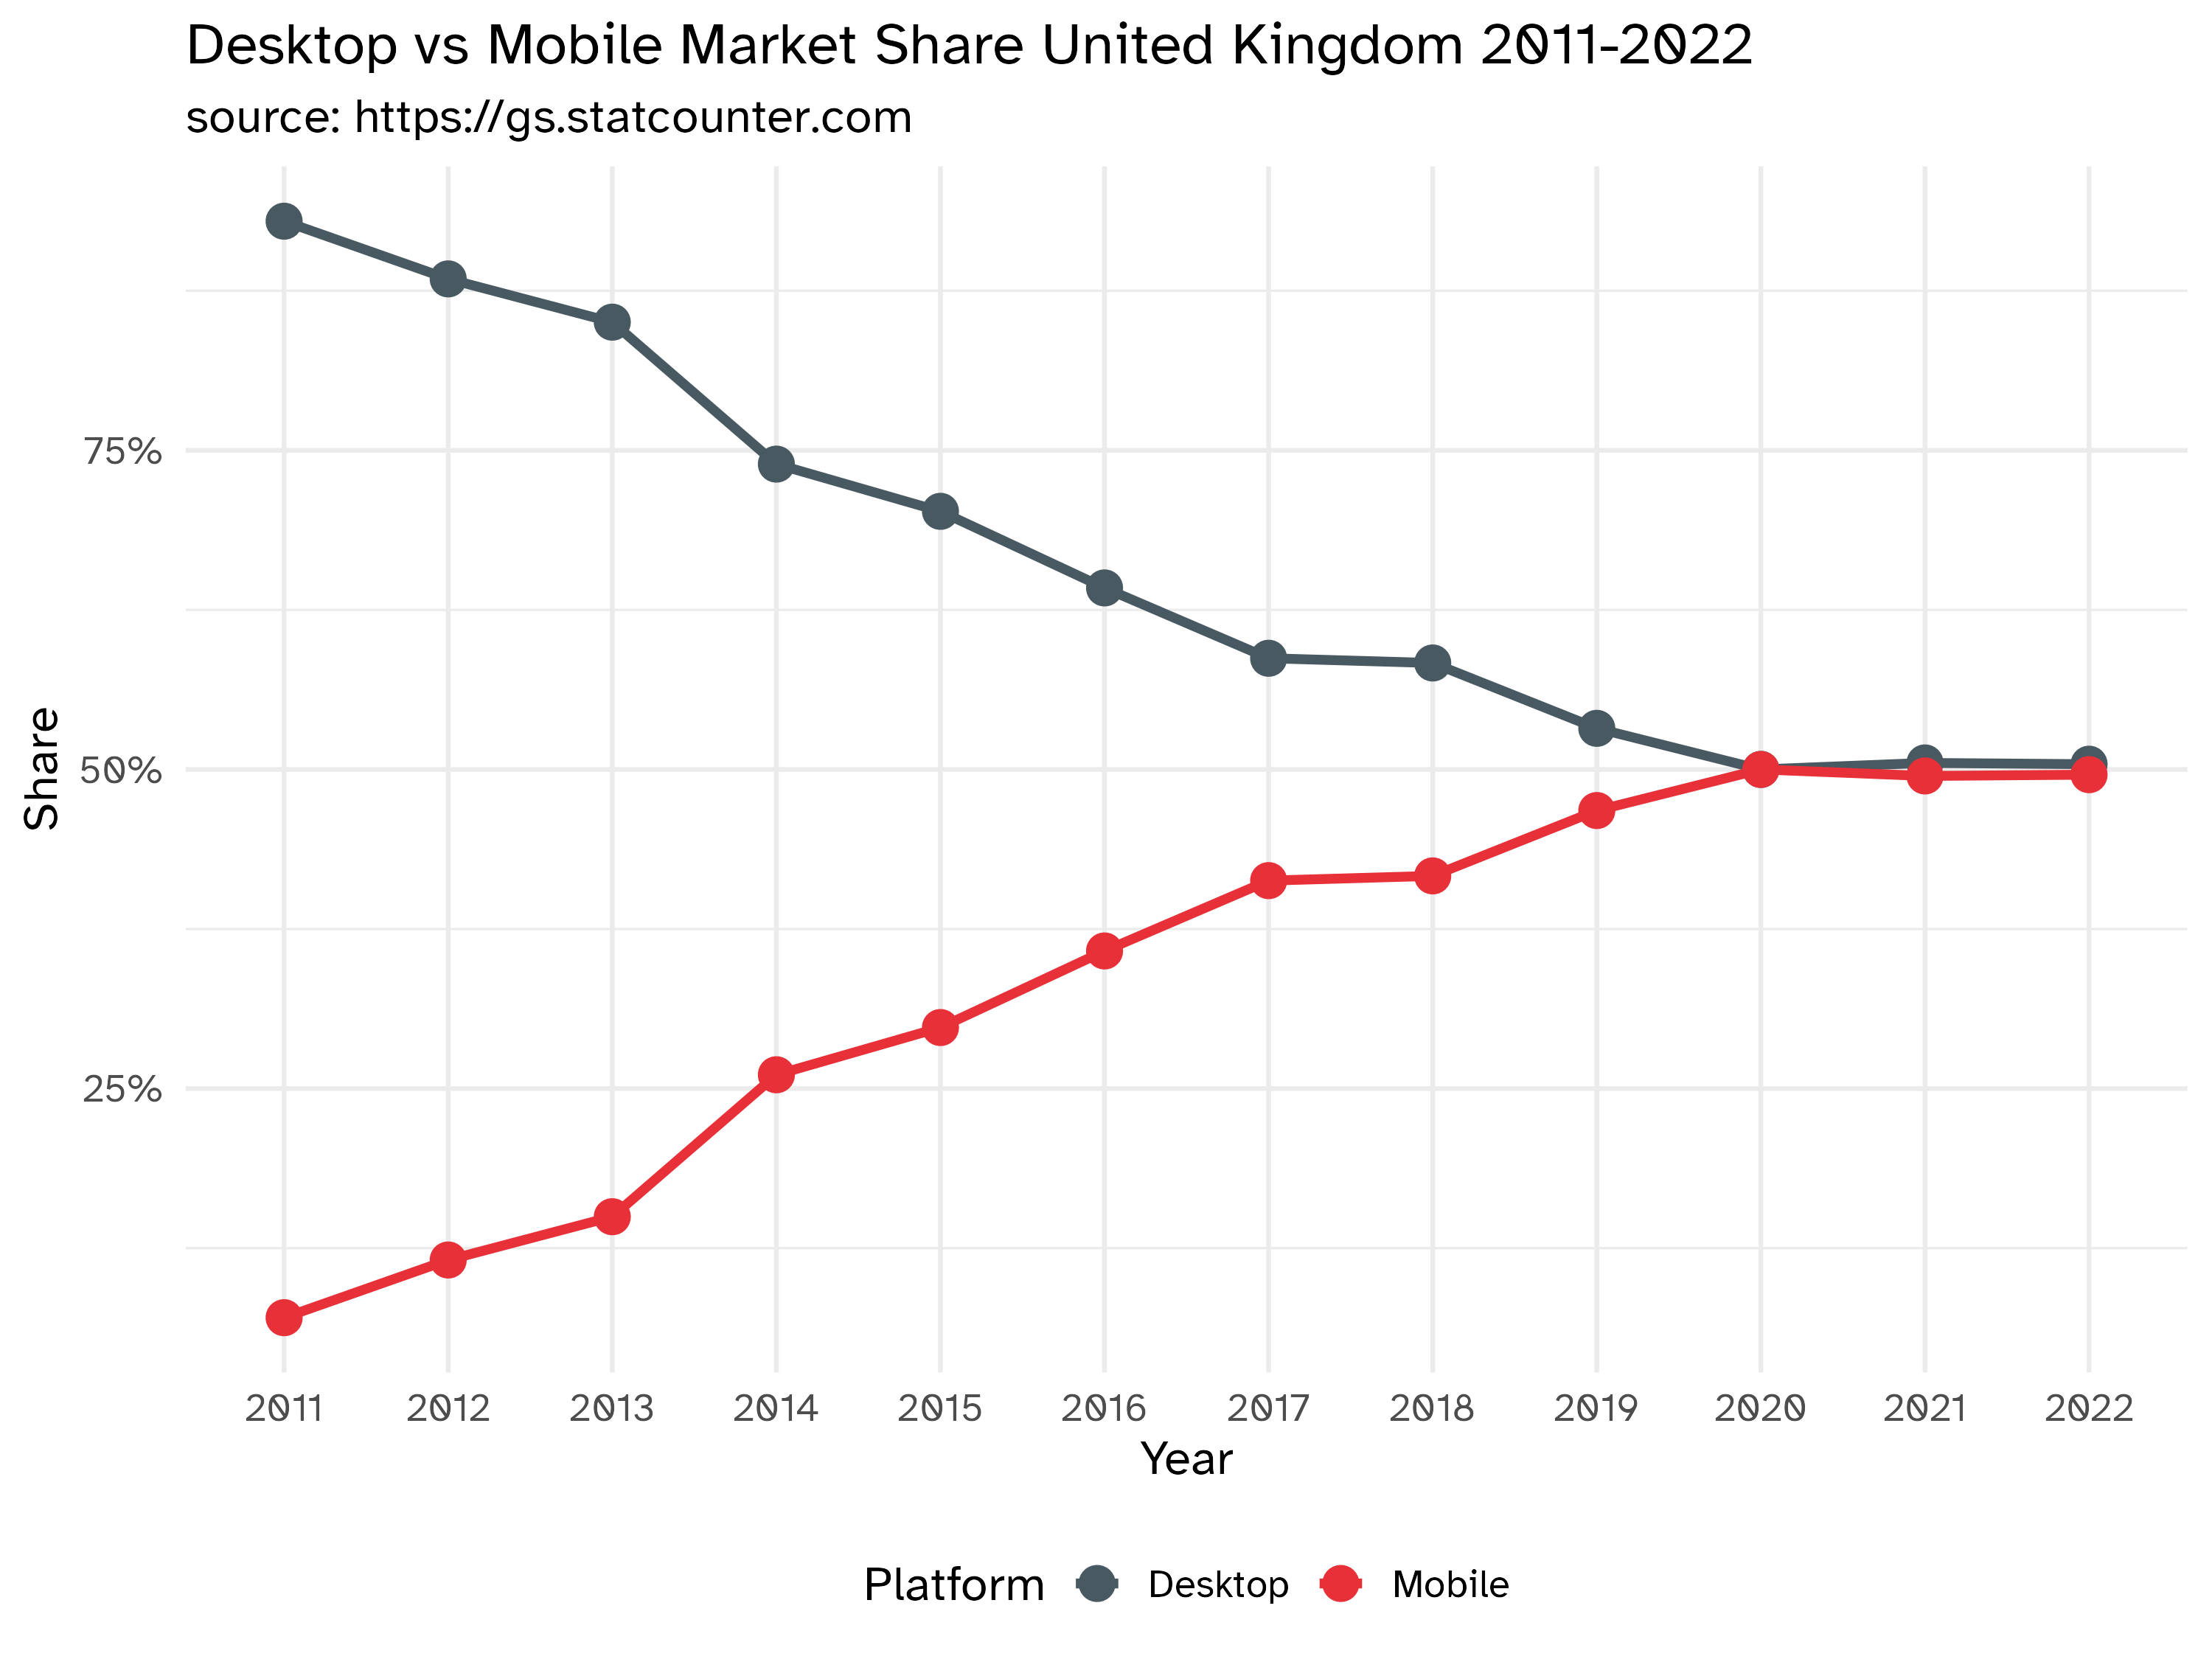
\includegraphics[width=10in,height=\textheight]{./img/uk-web-views-2011-2022.png}

}

\caption{\label{fig-uk-web-use}The world wide web turned 34 years old in
2023. The grey line shows the share of web views in the UK from desktop
computers and the red line shows the share of web views in the UK from
mobile devices.}

\end{figure}

\bookmarksetup{startatroot}

\hypertarget{what-to-read-instead}{%
\chapter{What to read instead}\label{what-to-read-instead}}

Nielsen Norman Group and Gov.uk

\url{https://www.nngroup.com/articles/how-users-read-on-the-web/}

\url{https://www.nngroup.com/topic/writing-web/}

\url{https://www.gov.uk/guidance/government-design-principles}

\url{https://www.gov.uk/guidance/content-design/writing-for-gov-uk}

\url{https://southampton.on.worldcat.org/oclc/798674328} Letting go of
the words Janice Redish

\bookmarksetup{startatroot}

\hypertarget{service-design}{%
\chapter{Service design}\label{service-design}}

\hypertarget{what-are-we-trying-to-achieve}{%
\section{What are we trying to
achieve?}\label{what-are-we-trying-to-achieve}}

\begin{figure}

{\centering 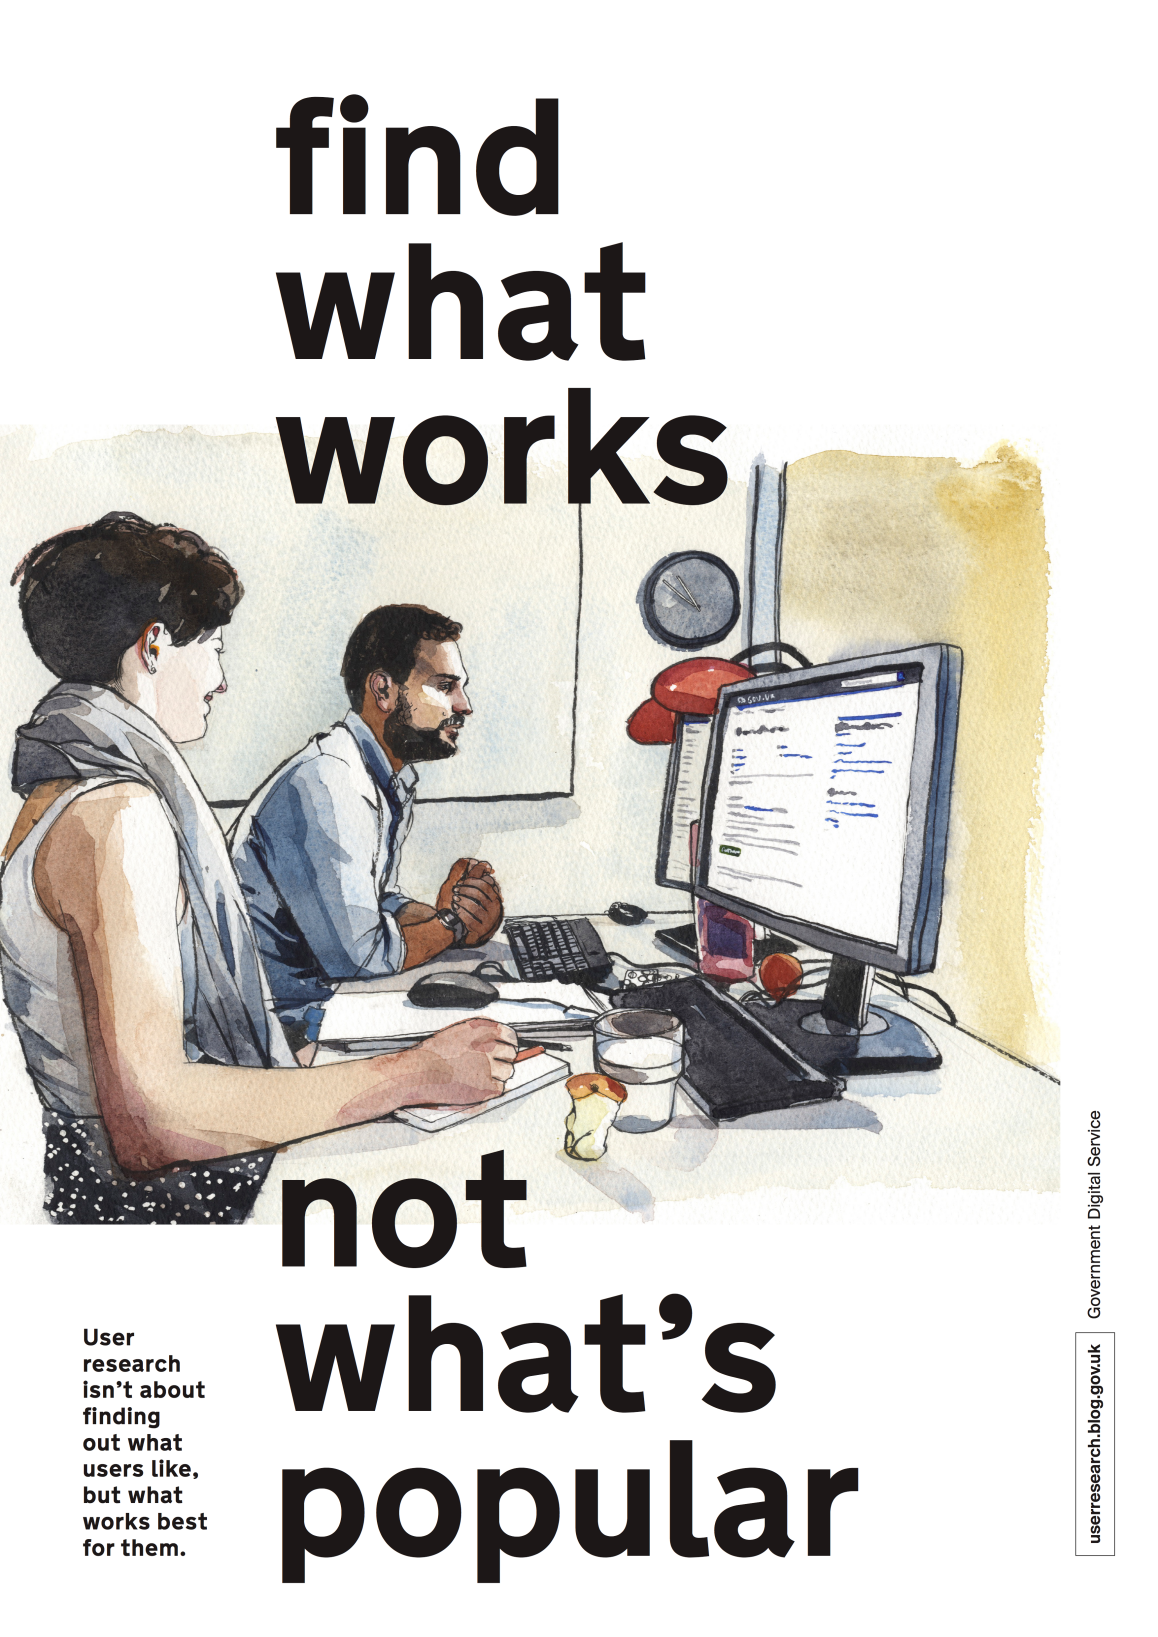
\includegraphics[width=3.86in,height=\textheight]{./img/small-gov.png}

}

\caption{\label{fig-find-what-works}Find What Works, Not What's Popular
poster, GOV.UK Government Digital Service
https://www.flickr.com/photos/gdsteam/20955195028}

\end{figure}

\hypertarget{optimisation-and-enshittification}{%
\section{Optimisation and
Enshittification}\label{optimisation-and-enshittification}}

This section can be skipped, but if you are interested in thinking more
about why web experience has got worse over time

\href{https://nothinghuman.substack.com/p/the-tyranny-of-the-marginal-user}{Ivan
Vendrov The Tyranny of the Marginal User}

\href{https://www.wired.com/story/tiktok-platforms-cory-doctorow/}{Cory
Doctorow on The `Enshittification' of TikTok}

\bookmarksetup{startatroot}

\hypertarget{how-do-people-read-webpages}{%
\chapter{How do people read
webpages?}\label{how-do-people-read-webpages}}

\hypertarget{whats-the-first-thing-we-do-on-landing-on-a-web-page}{%
\section{What's the first thing we do on landing on a web
page?}\label{whats-the-first-thing-we-do-on-landing-on-a-web-page}}

Check we are where we want to be! If not, we move on.

What does that imply about page design?

\hypertarget{what-is-the-difference-between-the-web-and-other-formats}{%
\section{What is the difference between the web and other
formats?}\label{what-is-the-difference-between-the-web-and-other-formats}}

\begin{itemize}
\item
  We scan in an F-pattern.
\item
  Long form (\textgreater1,000 words) we read in chunks, look for
  summaries, highlights or key-points.
\end{itemize}

\bookmarksetup{startatroot}

\hypertarget{writing-better-sentences}{%
\chapter{Writing better sentences}\label{writing-better-sentences}}

\hypertarget{how-do-we-improve-sentences}{%
\section{How do we improve
sentences?}\label{how-do-we-improve-sentences}}

Bennett Rules: https://www.earlymoderntexts.com/assets/jfb/bengor.pdf 1.
Verbs are better than nouns 2. Adverbs are better than adjectives 3.
Favour the Anglo-Saxon 4. Banish `very' and its ilk 5. Abstract nouns
should be fought like the devil 6. Avoid undue repetition 7. Be careful
with commas. 8. Attend to the sound

\bookmarksetup{startatroot}

\hypertarget{using-imagery-and-visuals}{%
\chapter{Using imagery and visuals}\label{using-imagery-and-visuals}}

\hypertarget{why-would-we-use-visuals}{%
\section{Why would we use visuals?}\label{why-would-we-use-visuals}}

\begin{itemize}
\item
  To impart information that cannot be easily expressed in words
  e.g.~trends.
\item
  To create ambience.
\end{itemize}

\hypertarget{why-would-we-not-use-visuals}{%
\section{Why would we not use
visuals?}\label{why-would-we-not-use-visuals}}

\begin{itemize}
\tightlist
\item
  They make scanning more difficult, especially on mobile devices.
\end{itemize}

\bookmarksetup{startatroot}

\hypertarget{references}{%
\chapter*{References}\label{references}}
\addcontentsline{toc}{chapter}{References}

\markboth{References}{References}

\hypertarget{refs}{}
\begin{CSLReferences}{0}{0}
\end{CSLReferences}



\end{document}
